\uuid{UKuS}
\exo7id{7139}
\titre{exo7 7139}
\auteur{megy}
\organisation{exo7}
\datecreate{2017-04-05}
\isIndication{true}
\isCorrection{true}
\chapitre{Géométrie affine euclidienne}
\sousChapitre{Géométrie affine euclidienne du plan}
\module{Géométrie}
\niveau{L2}
\difficulte{}

\contenu{
\texte{
Soit $ABC$ un triangle, $H$ son orthocentre et $\mathcal C$ son cercle circonscrit. La hauteur issue de $B$ recoupe $\mathcal C$ en $H'$. Montrer que $H'$ est le symétrique de $H$ par rapport à la droite $(AC)$. 

\begin{center}
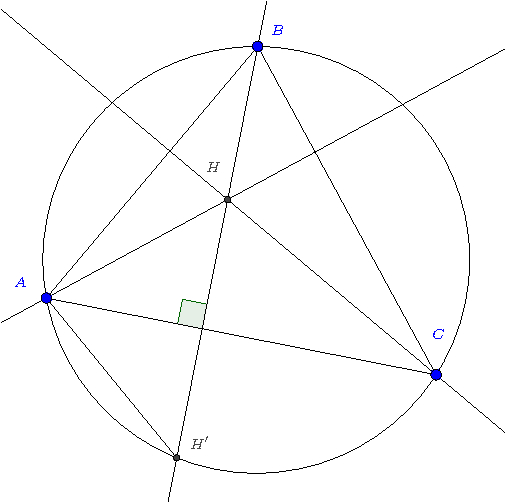
\includegraphics{../images/pdf/UKuS-1.pdf}
\end{center}
}
\indication{Utiliser les différentes caractérisations des triangles isocèles.}
\reponse{
Si $ABC$ est rectangle, l'orthocentre coïncide avec un des sommets et la vérification de l'assertion est relativement facile. Dans la suite on suppose qu'on n'est pas dans ce cas.

Par définition, $H'$ est le symétrique de $H$ par rapport à $(AC)$ si $(AC)$ est la médiatrice de $[HH']$. C'est cela qu'on doit montrer.



D'autre part, par définition, on a $(AC) \bot (HH')$, donc $(AC)$ est la hauteur de $AHH'$ issue de $A$. 

Donc si $AHH'$ est isocèle en $A$, alors cette hauteur de $AHH'$  est aussi la médiane issue de $A$ et c'est encore la médiatrice du côté opposé à $A$ c'est-à-dire $[HH']$.

Il suffit donc de montrer que $AHH'$ est isocèle en $A$. Pour cela, il suffit de montrer que les angles adjacents à la base sont égaux, autrement dit $\widehat{AHH'} = \widehat{AH'H}$ avec des angles géométriques non orientés, ou plus précisément avec des angles orientés $(H'A,H'H)=(HH',AH)$.

Suivant la méthodologie habituelle, on marque de façon systématique les angles égaux (ou complémentaires, supplémentaires etc) sur la figure. Ceci indique la marche à suivre pour la preuve.


\begin{center}
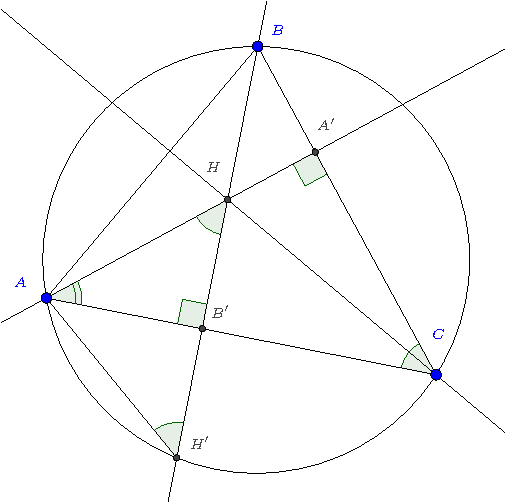
\includegraphics{../images/pdf/UKuS-2.pdf}
\end{center}

Montrons que $(H'A,H'H)=(HH',AH)$. On a :
\begin{align*}
(H'A,H'H) &= (H'A,H'B) \text{ (car $(H'H)=(HB)$}\\
&= (CA,CB) \text{ (car $ABCH'$ est inscriptible)}\\
&= (CA,AH)+(AH,CB) \text{ (par Chasles)}\\
&= (CA,AH)+\pi/2 \text{ (car $(AH)$ est une hauteur de $ABC$)}\\
&= (CA,AH)+(HH',CA)\\
&= (HH',AH) \text{ (par Chasles)}
\end{align*}
}
}
